\documentclass[a4paper,12pt]{article}
\usepackage[english]{babel}
\usepackage{multicol}
\usepackage{caption}
\usepackage{hyperref}
\usepackage{graphicx}


\begin{document}
\title{Projects Dashboard \\ \vspace{2 mm} {\large Track, analyze and
decide}}

\author{H\'{e}ctor L\'{o}pez Sacanell \\
	\small Universitat de Lleida - Escola Polit\`{e}cnica Superior \\
	\small \texttt{\href{mailto:hlopez1@alumnes.udl.es}{hlopez1@alumnes.udl.es}}}

\maketitle
\begin{abstract}
Project management is an open discipline that allows companies to drive their
market solutions to the success. Those disciplines can be standard or \emph{ad
hoc}, and it depends on their needs. In my case, I see room for improvement on
project management and make the process direct and easy with no stress in the
team, making it more efficient only applying the right key performance
indicators and showing data in the right way to be analyzed.
\end{abstract}

\begin{multicols}{2}

\section{Motivation}
When you need to drive few projects at the same time and rule more than one
country with specific needs and requirements, you cannot only manage those
projects, you need to \textbf{master} them!

Wikipedia defines project management as \emph{``the discipline of
planning, organizing, motivating, and controlling resources to achieve specific
goals.''}\footnote{\url{http://en.wikipedia.org/wiki/Project\_management}}.
And in order to success on this journey, computer science can help you
automating part of the process and show data in a way that fits your needs to
take the best decision.

Automating is the key. Let computers do the hard work, so we can 
spend more time learning from the past and improve our methodologies.


\section{Introduction}
One of the most required topics when you are managing few projects at the same 
time, is to have a wide view about what is the current situation and what will
come next.
Defining a global roadmap solves the point to have visibility about what are next 
expected projects, but only with that is not enough to have a quick view
about how far we are from the original timeline (\emph{variance}).

In order to calculate this variance, you need to measure performance of your
projects. This measure is not always easy to calculate, but it depends on how
deep you look for.

If you start from the basement, breaking down the project deeply, then you
will find a lot of obstacles to solve before getting something ready, and it
will quickly make you to loose the point. Like, the time you need to spend getting effort
from all small components, that is the easiest part, but also to track them
during the development.

Although, you can try to start from the top, and apply solutions for the small
challenges you are getting from lower levels. Following this approach you don't 
loose the main objective, an also you can feel confident because giving small
solutions, usually with small effort, leaves the rest of your time to analyze
and decide.

\section{Process and Methodoloy}
There is a big amount of project management methodologies. From those that are
very restrictive, to the ones that make you live in a free and self driven
management. This wide variety of methodologies (standard and \emph{ad hoc})
exist because of teams needs, and they just give the right solution for
the specific problem. Choosing one that fits into your case, makes you happy
and efficient. But leaving aside specific process and taking out the main concept,
all methodologies plan the tasks to do, how to carry them out, track and learn
from them, iteratively within the same project or with different ones (see diagram
\ref{figure:process}).

\begin{center}
	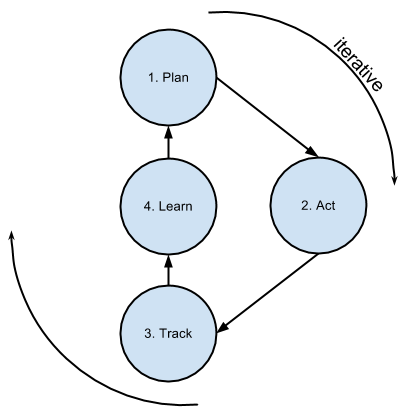
\includegraphics[width=0.5\textwidth]{resources/process.png}
	\captionof{figure}{Key steps in any project methodology}
	\label{figure:process}
\end{center}

Besides, the step from tracking to learn is the key and the first topic of this
project. We need to spend some time evaluating \emph{what} we want to learn and
what we are going to track (KPI\footnote{Key Performance Indicator}).
Once we have it clear, then we need to decide \emph{how} we are going to implement them.

Once we have solved the first problem, then we only need to show the right
information and KPIs in order to analyzed them and improve the process. And this is the
second part of the project.

\section{The Problem}
Force the team to follow a specific process to help you to track and the team to
learn is not always the right decision, because it could not match team's
ideosyncracy. So, we need to do it in the other way around, understanding how
the team behaves and defining a custom process that fits on it, aiming the same
objective.

As soon as you start getting data, next step is to show it in the right way, so
team and managers can get the required information in an easy and a clear way.

\section{The Proposal}
There are many world-wide solutions that help project managers to work with
mentioned performance indicators, such as MS Project, tracking tools
like Jira and Redmine. But, those tools require the team to start working on
them from scratch, and benefits will not be visible until few projects, and you
will also face some problems that could block you to adapt the team to new
software. That's why, the proposed approach is to start from the top and manage
issues from the top level to the ground, showing the team points to improve and
get from the team suggestions and solutions to the specific problems. Building
and adapting the tool to the team.

Defining a clean dashboard where you can see, in different sections, selected
performance indicators. Having a quick view about what is going on and what is
scheduled. Having also the possibility to go down to understand causes of the
variance in order to define, and track, the key learning and apply it on the
next iteration or project.

Architecture defined for this dashboard is to isolate and decouple data from
business logic and presentation. This will give the flexibility to process and
show the same information using different technologies, based on the end user's
device.

Isolating data from business logic will allow us to use different technologies
to process it, making flexible and defining and strong scalability in order to get
quick results and prototypes from the beginnig (see high level flow
\ref{figure:architecture}).

\end{multicols}
\begin{center}
	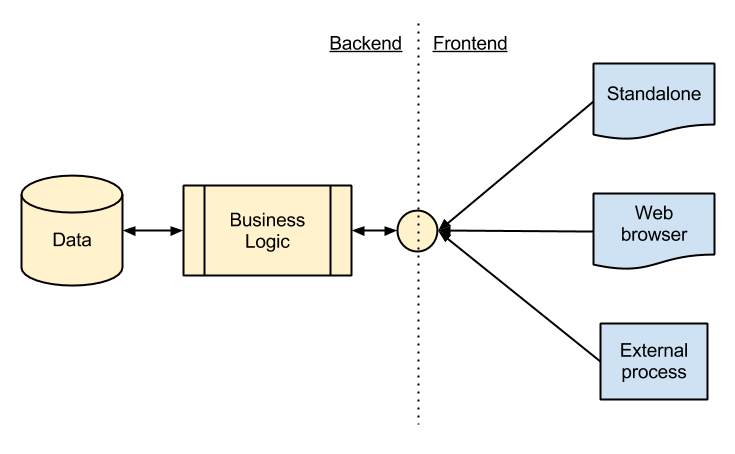
\includegraphics[width=1.0\textwidth]{resources/architecture.png}
	\captionof{figure}{Proposed architecture}
	\label{figure:architecture}
\end{center}

\end{document}
